\documentclass[conference]{IEEEtran}
\IEEEoverridecommandlockouts
% The preceding line is only needed to identify funding in the first footnote. If that is unneeded, please comment it out.

\usepackage{cite}
\usepackage{amsmath,amssymb,amsfonts}
\usepackage{algorithmic}
\usepackage{graphicx}
\usepackage{textcomp}
\usepackage{xcolor}
\def\BibTeX{{\rm B\kern-.05em{\sc i\kern-.025em b}\kern-.08em
    T\kern-.1667em\lower.7ex\hbox{E}\kern-.125emX}}
    
\begin{document}

\title{Biophysical Mechanisms of Photosynthesis and Perspectives for Artificial Energy Conversion}

\author{\IEEEauthorblockN{Luka Tadic}
\IEEEauthorblockA{\textit{Electrical Energy Systems and Electromobility (M.Sc.)} \\
\textit{Technische Hochschule Ulm (THU)}\\
Ulm, Germany \\
tadilu01@thu.de} % Hier deine echte Hochschul-E-Mail eintragen
}

\maketitle

\begin{abstract}
This paper explores the biophysical mechanisms of natural photosynthesis with a strong focus on technical and engineering perspectives. As global energy demands rise, biological processes like light harvesting, electron transport, and carbon fixation offer blueprints for highly efficient energy conversion systems. We analyze the thylakoid membrane as a nanoscale solar module and the electron transport chain as a biological circuit. Furthermore, process efficiencies and thermodynamic limits are evaluated. Finally, the transition from natural principles to artificial photosynthesis, such as photoelectrochemical cells for green hydrogen production, is discussed.
\end{abstract}

\begin{IEEEkeywords}
Photosynthesis, Electron Transport, Bio-inspired Engineering, Energy Conversion, Artificial Leaf
\end{IEEEkeywords}

\section{Introduction}
% Motivation: Energiebedarf der Menschheit und biologische Vorbilder
% Kurzer Überblick: Was ist Photosynthese aus technischer Sicht?
% Ziel des Papers
This section will introduce the global energy challenge and the motivation to look at natural photosynthesis from an engineering perspective. It sets the scope of the paper, emphasizing the technical mechanisms rather than purely biological aspects.

\section{Biophysical Principles of Light Harvesting}
\subsection{The Thylakoid Membrane as a Solar Module}
% Aufbau der Struktur
Here, you can describe the physical structure of the membrane acting similarly to a semiconductor or solar cell.

\subsection{Antenna Complexes and Exciton Transfer}
% Exzitonen-Transfer (Energieübertragung auf technischer Ebene)
Discuss the quantum mechanical and biophysical energy transfer mechanisms.

\begin{figure}[htbp]
\centerline{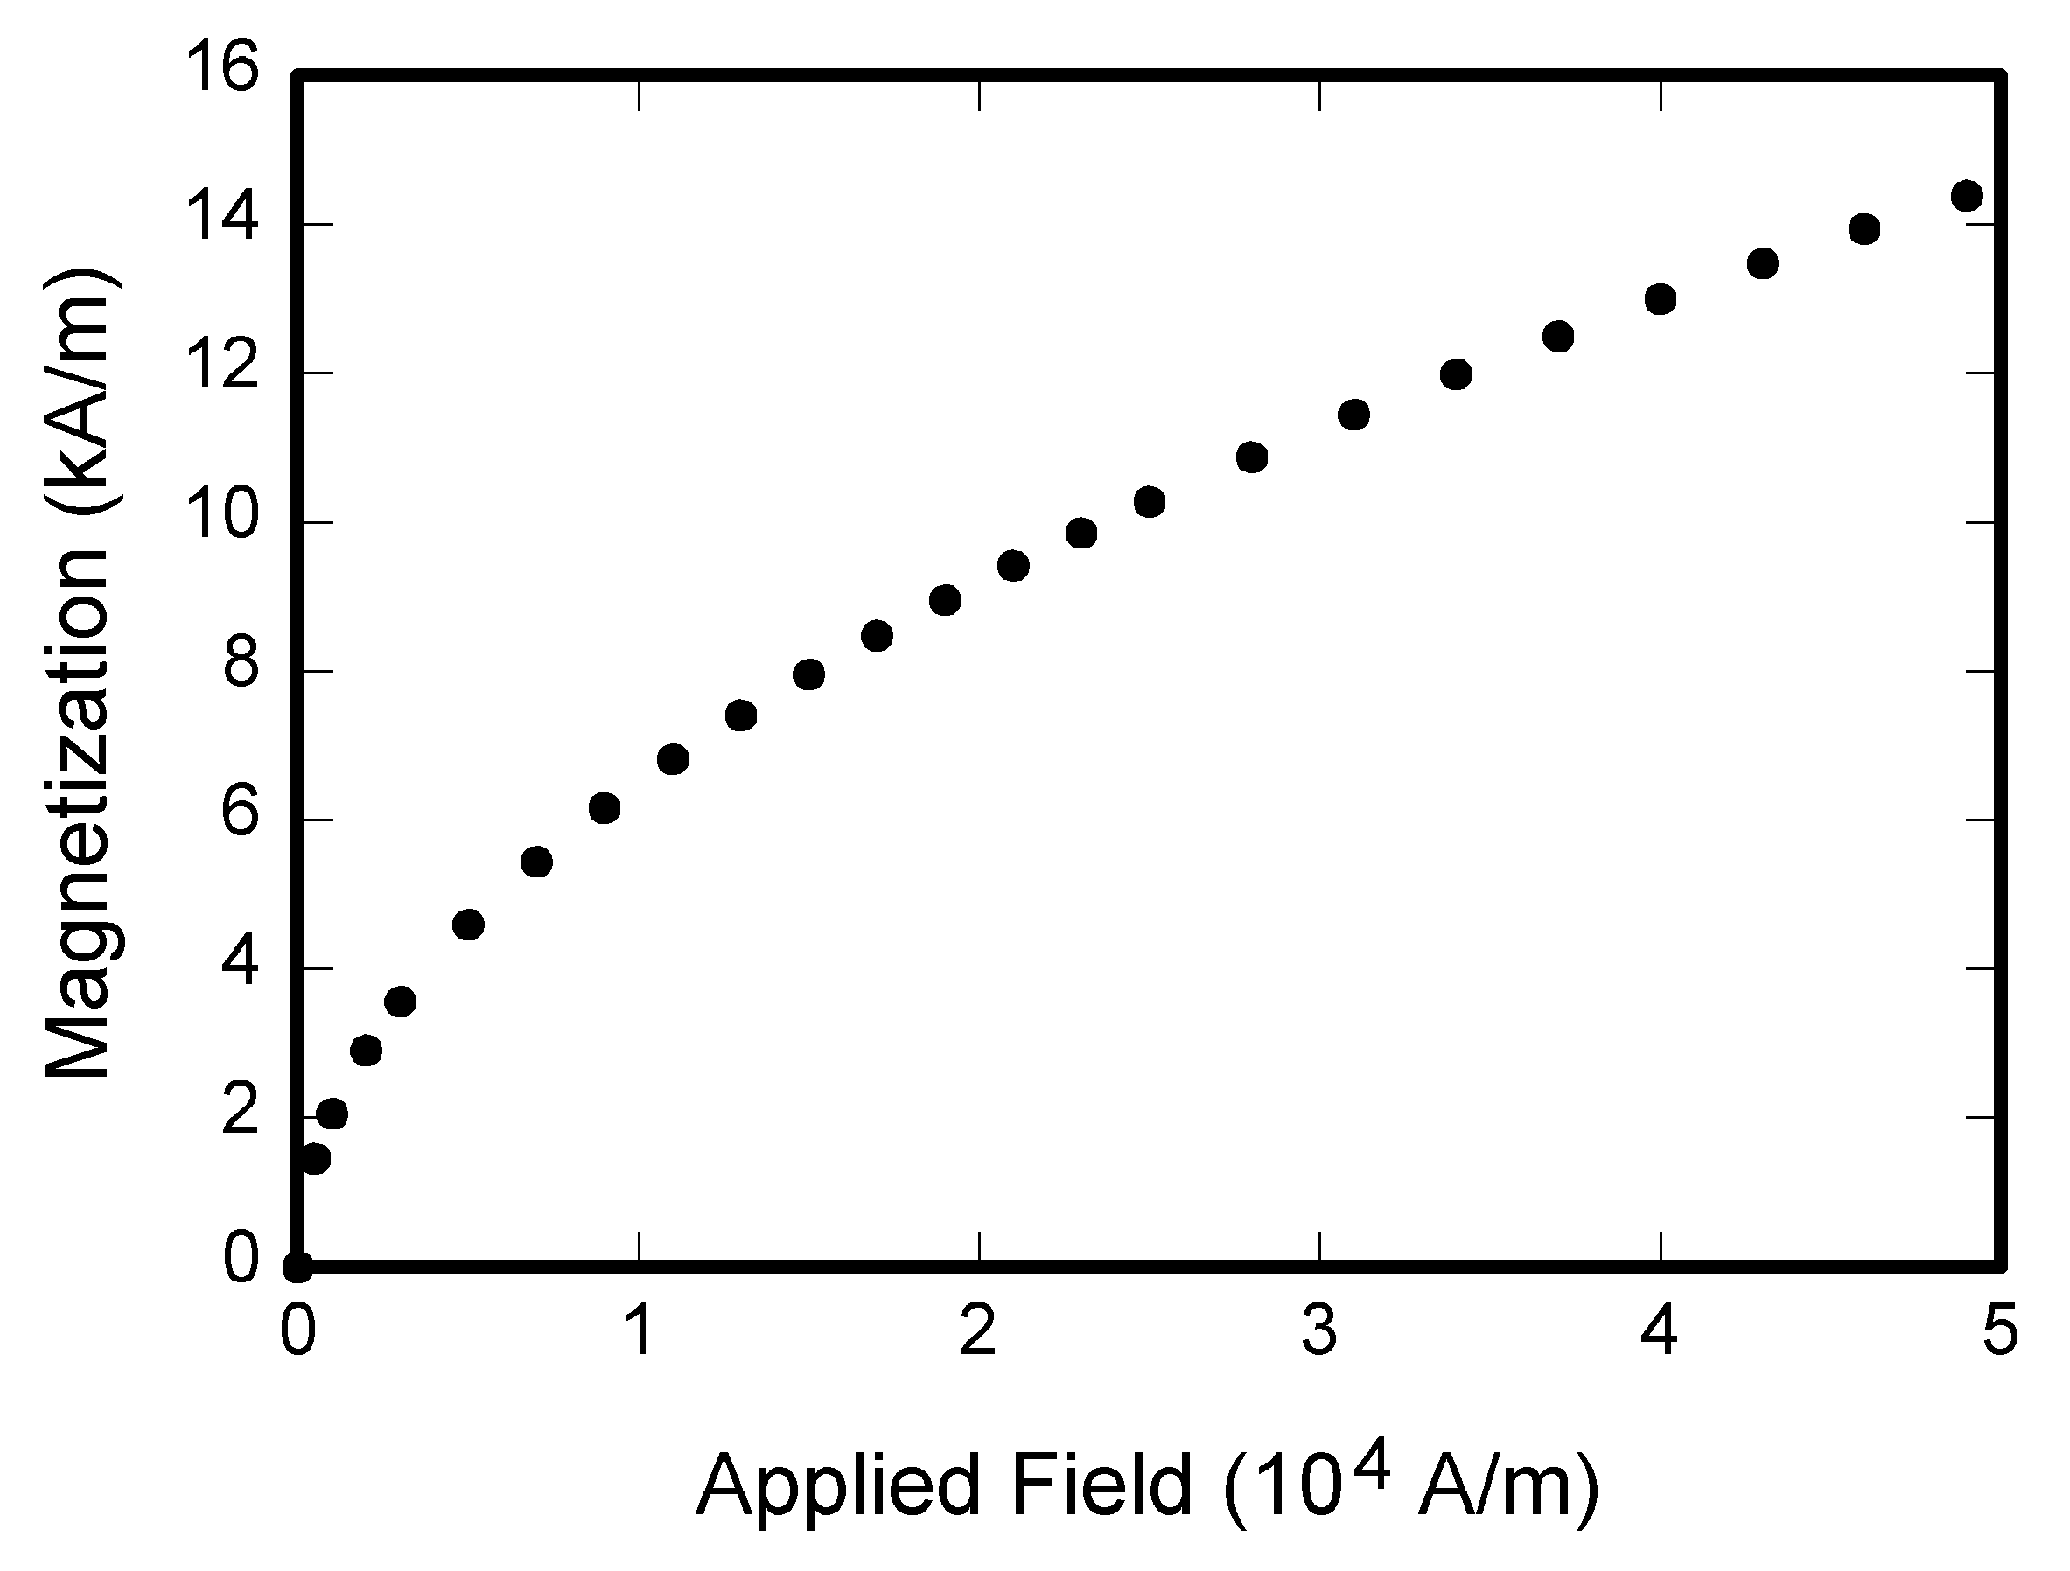
\includegraphics[width=0.45\textwidth]{images/fig1.png}} % Ersetze fig1.png mit deinem Bild
\caption{Schematic representation of light-harvesting antenna complexes and energy transfer.}
\label{fig:antenna}
\end{figure}

\section{The Electron Transport Chain as a Biological Circuit}
\subsection{Photosystem II and Photolysis}
% Wasserspaltung (Photolyse) als elektrochemischer Prozess
Detail the electrochemical water splitting process.

\subsection{Cytochrome and Photosystem I}
Tracing the electron flow as a current through a biological circuit. 

\begin{figure}[htbp]
\centerline{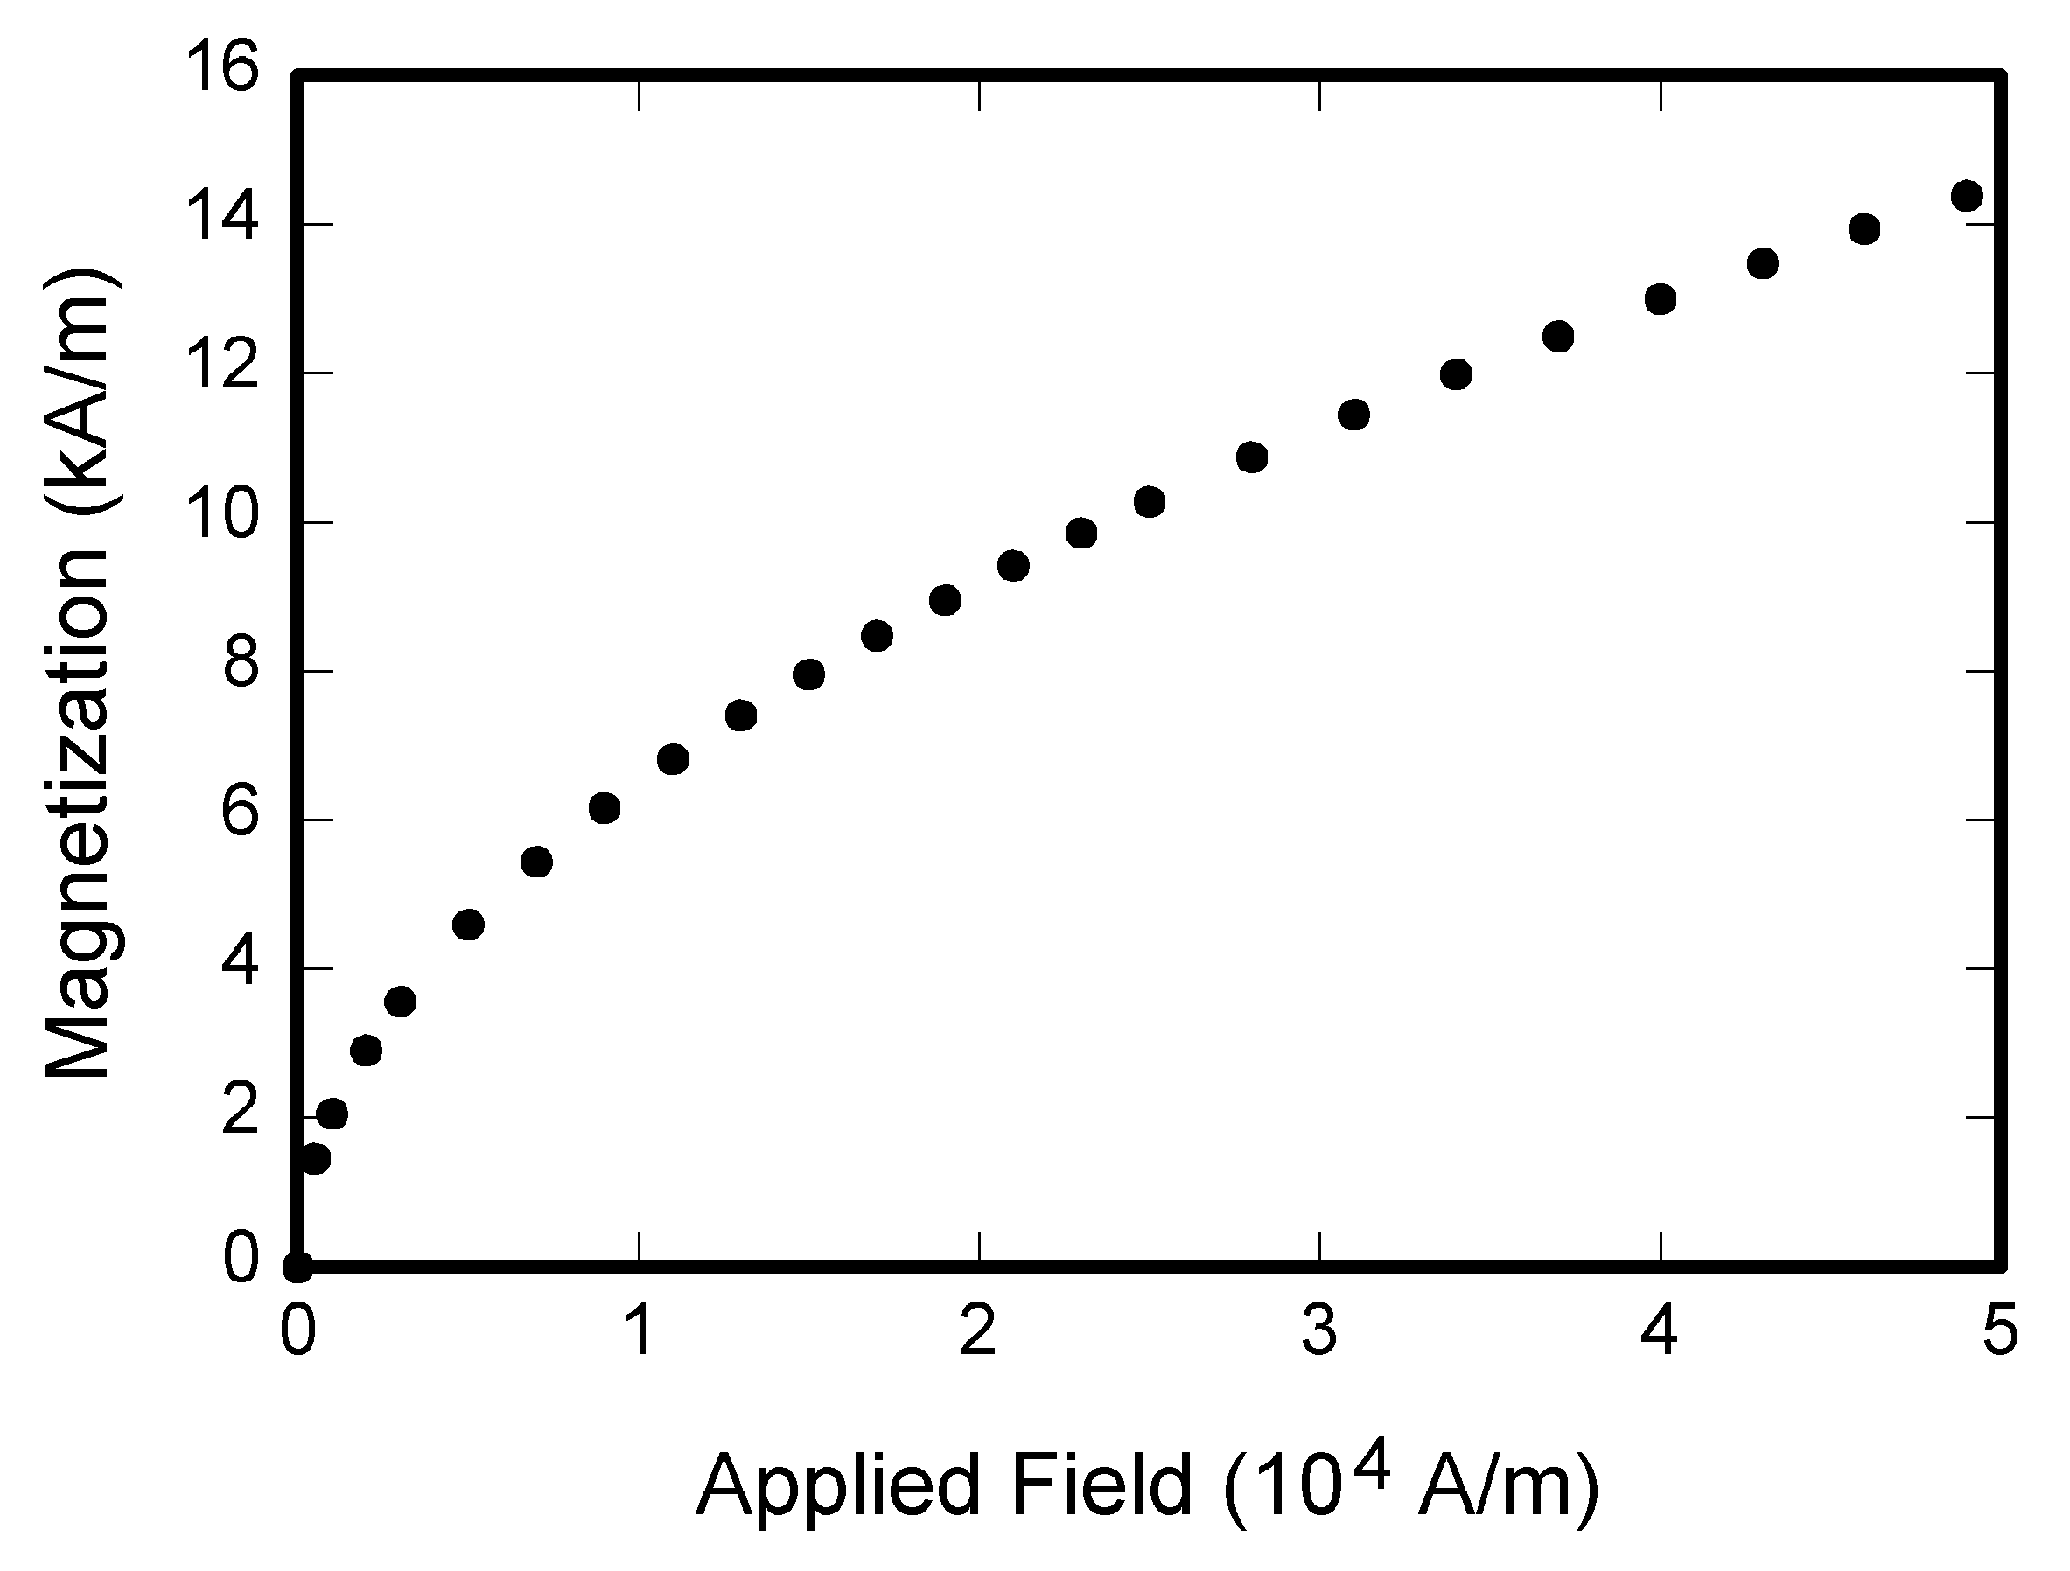
\includegraphics[width=0.45\textwidth]{images/fig1.png}} 
\caption{The Z-scheme of electron transport modeled as an energetic circuit.}
\label{fig:zscheme}
\end{figure}

\subsection{ATP Synthase: A Biological Motor}
% Mechanische Rotation zur chemischen Energiespeicherung
Explain the chemo-mechanical rotation mechanism of ATP synthase.

\begin{figure}[htbp]
\centerline{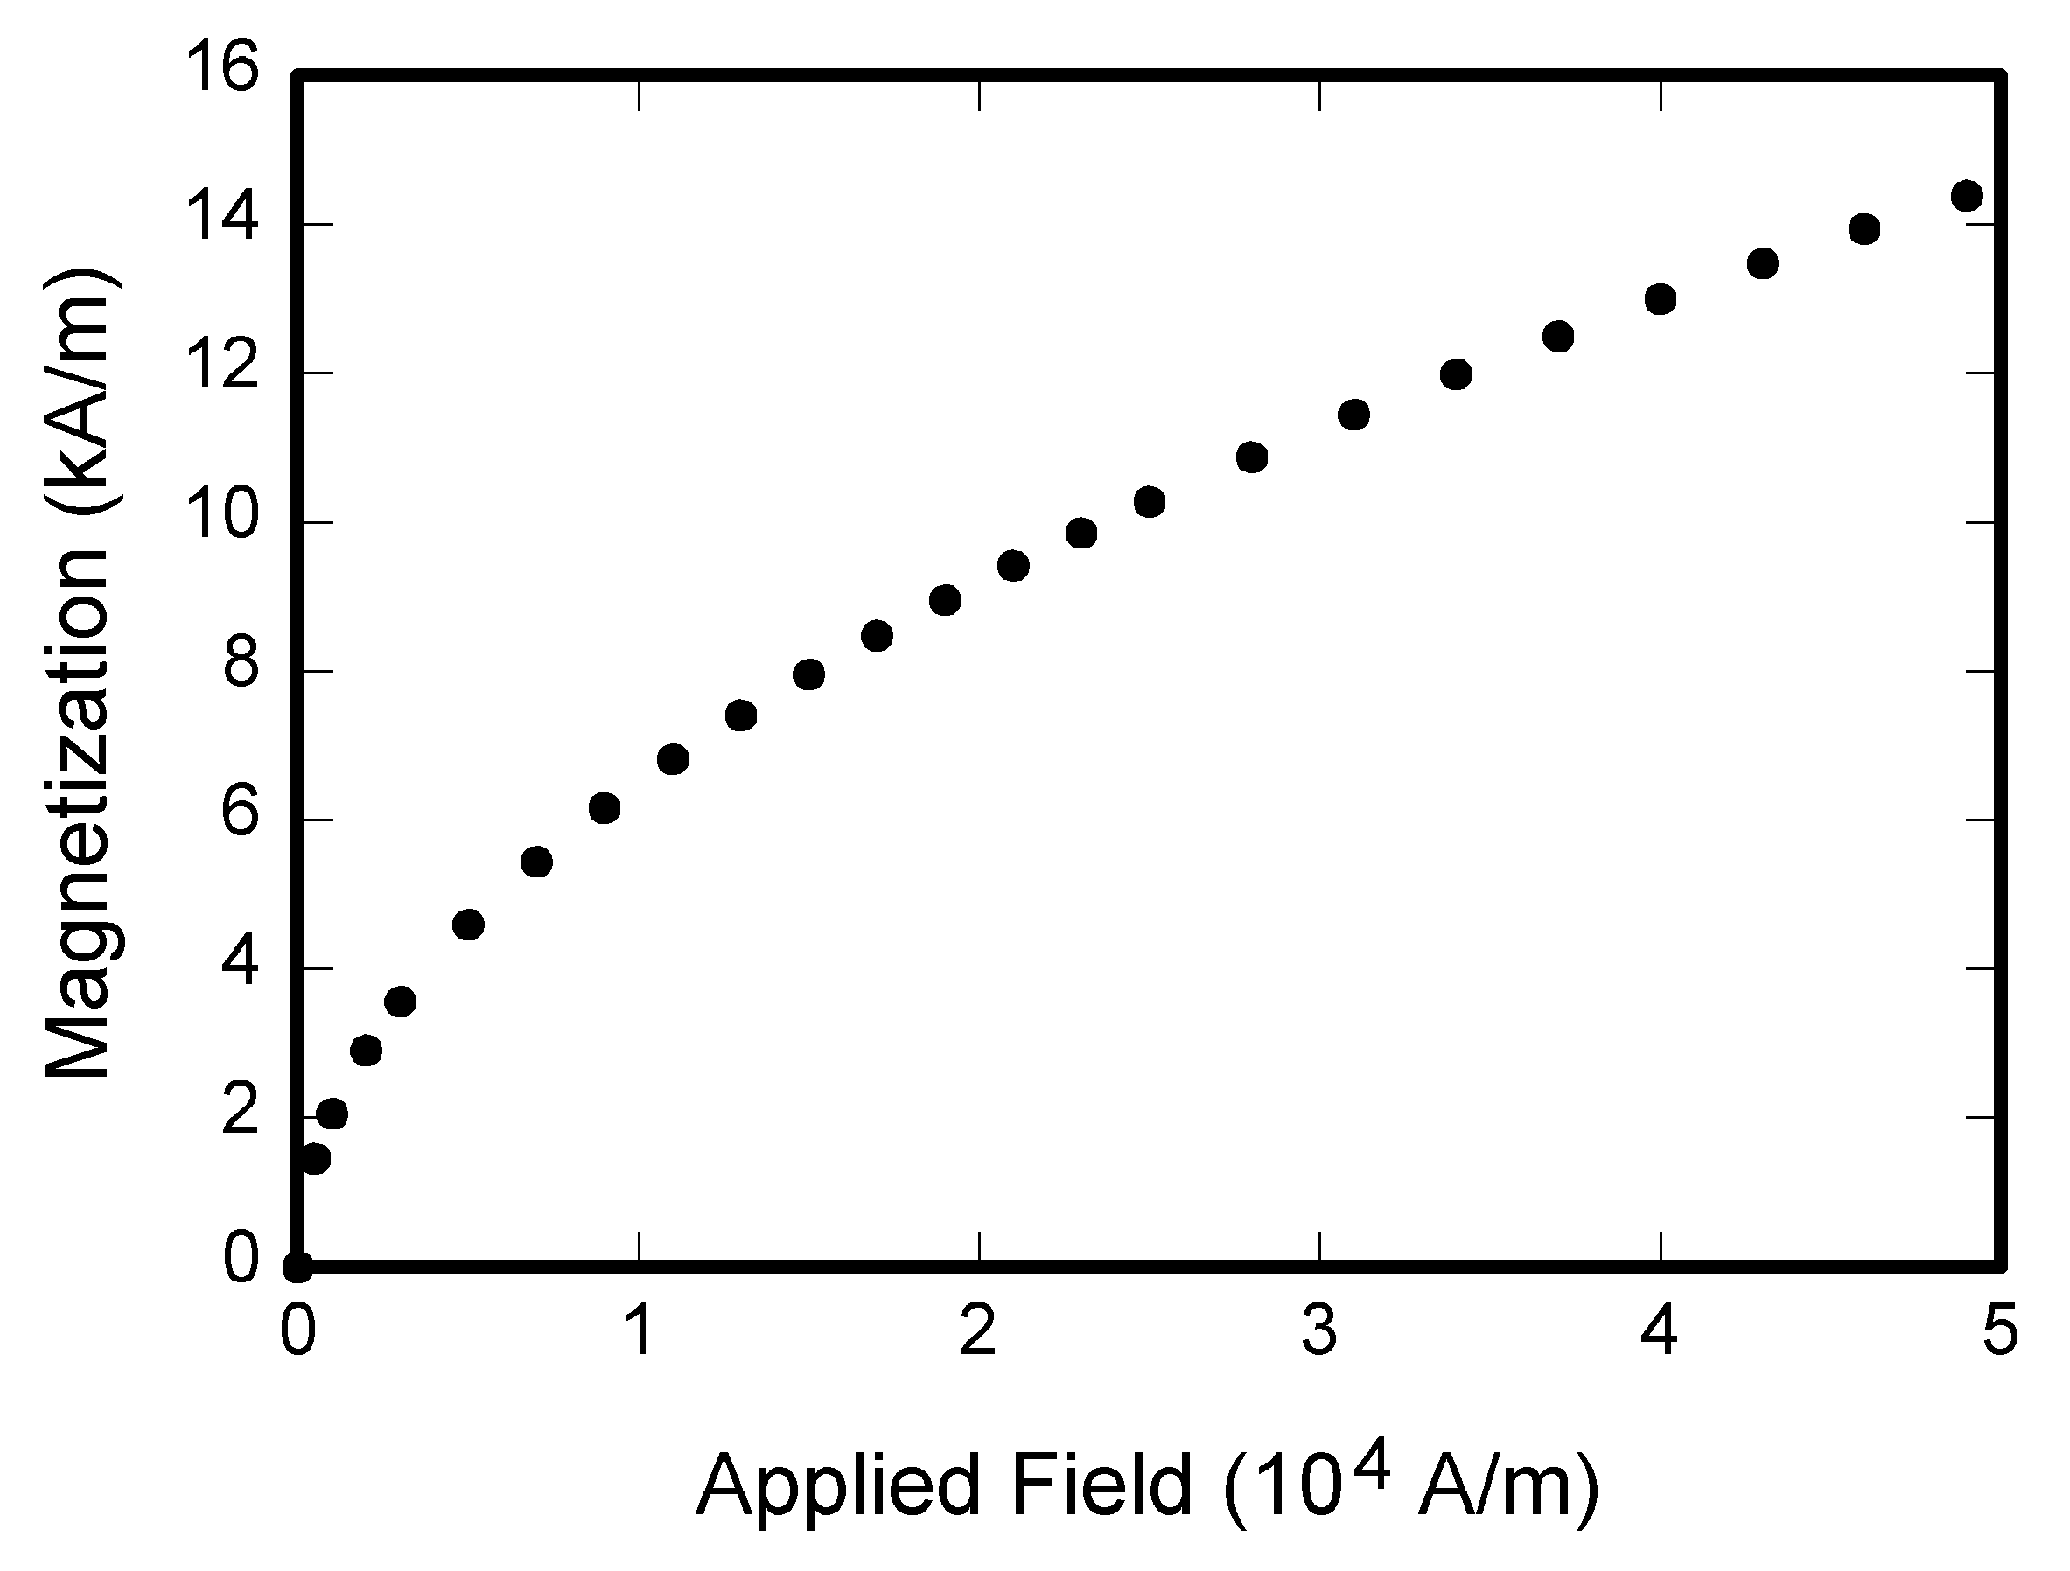
\includegraphics[width=0.45\textwidth]{images/fig1.png}} 
\caption{Structural mechanics and rotation of the ATP synthase complex.}
\label{fig:atpsynthase}
\end{figure}

\section{Carbon Fixation and Process Efficiency}
\subsection{The Calvin Cycle as a Catalytic Loop}
Describe the dark reaction as an industrial-like catalytic cycle \cite{Photosynthese2026}.

\subsection{Thermodynamic Limits and Efficiency}
% Wirkungsgrad und thermodynamische Grenzen
Analyze the overall energy efficiency of natural photosynthesis compared to technical limits (e.g., Shockley-Queisser limit).

\section{Transition to Artificial Photosynthesis}
\subsection{Photoelectrochemical Cells}
% Technische Nachbildung der Wasserspaltung
Explain how engineers mimic the natural Z-scheme using semiconductors and catalysts.

\begin{figure}[htbp]
\centerline{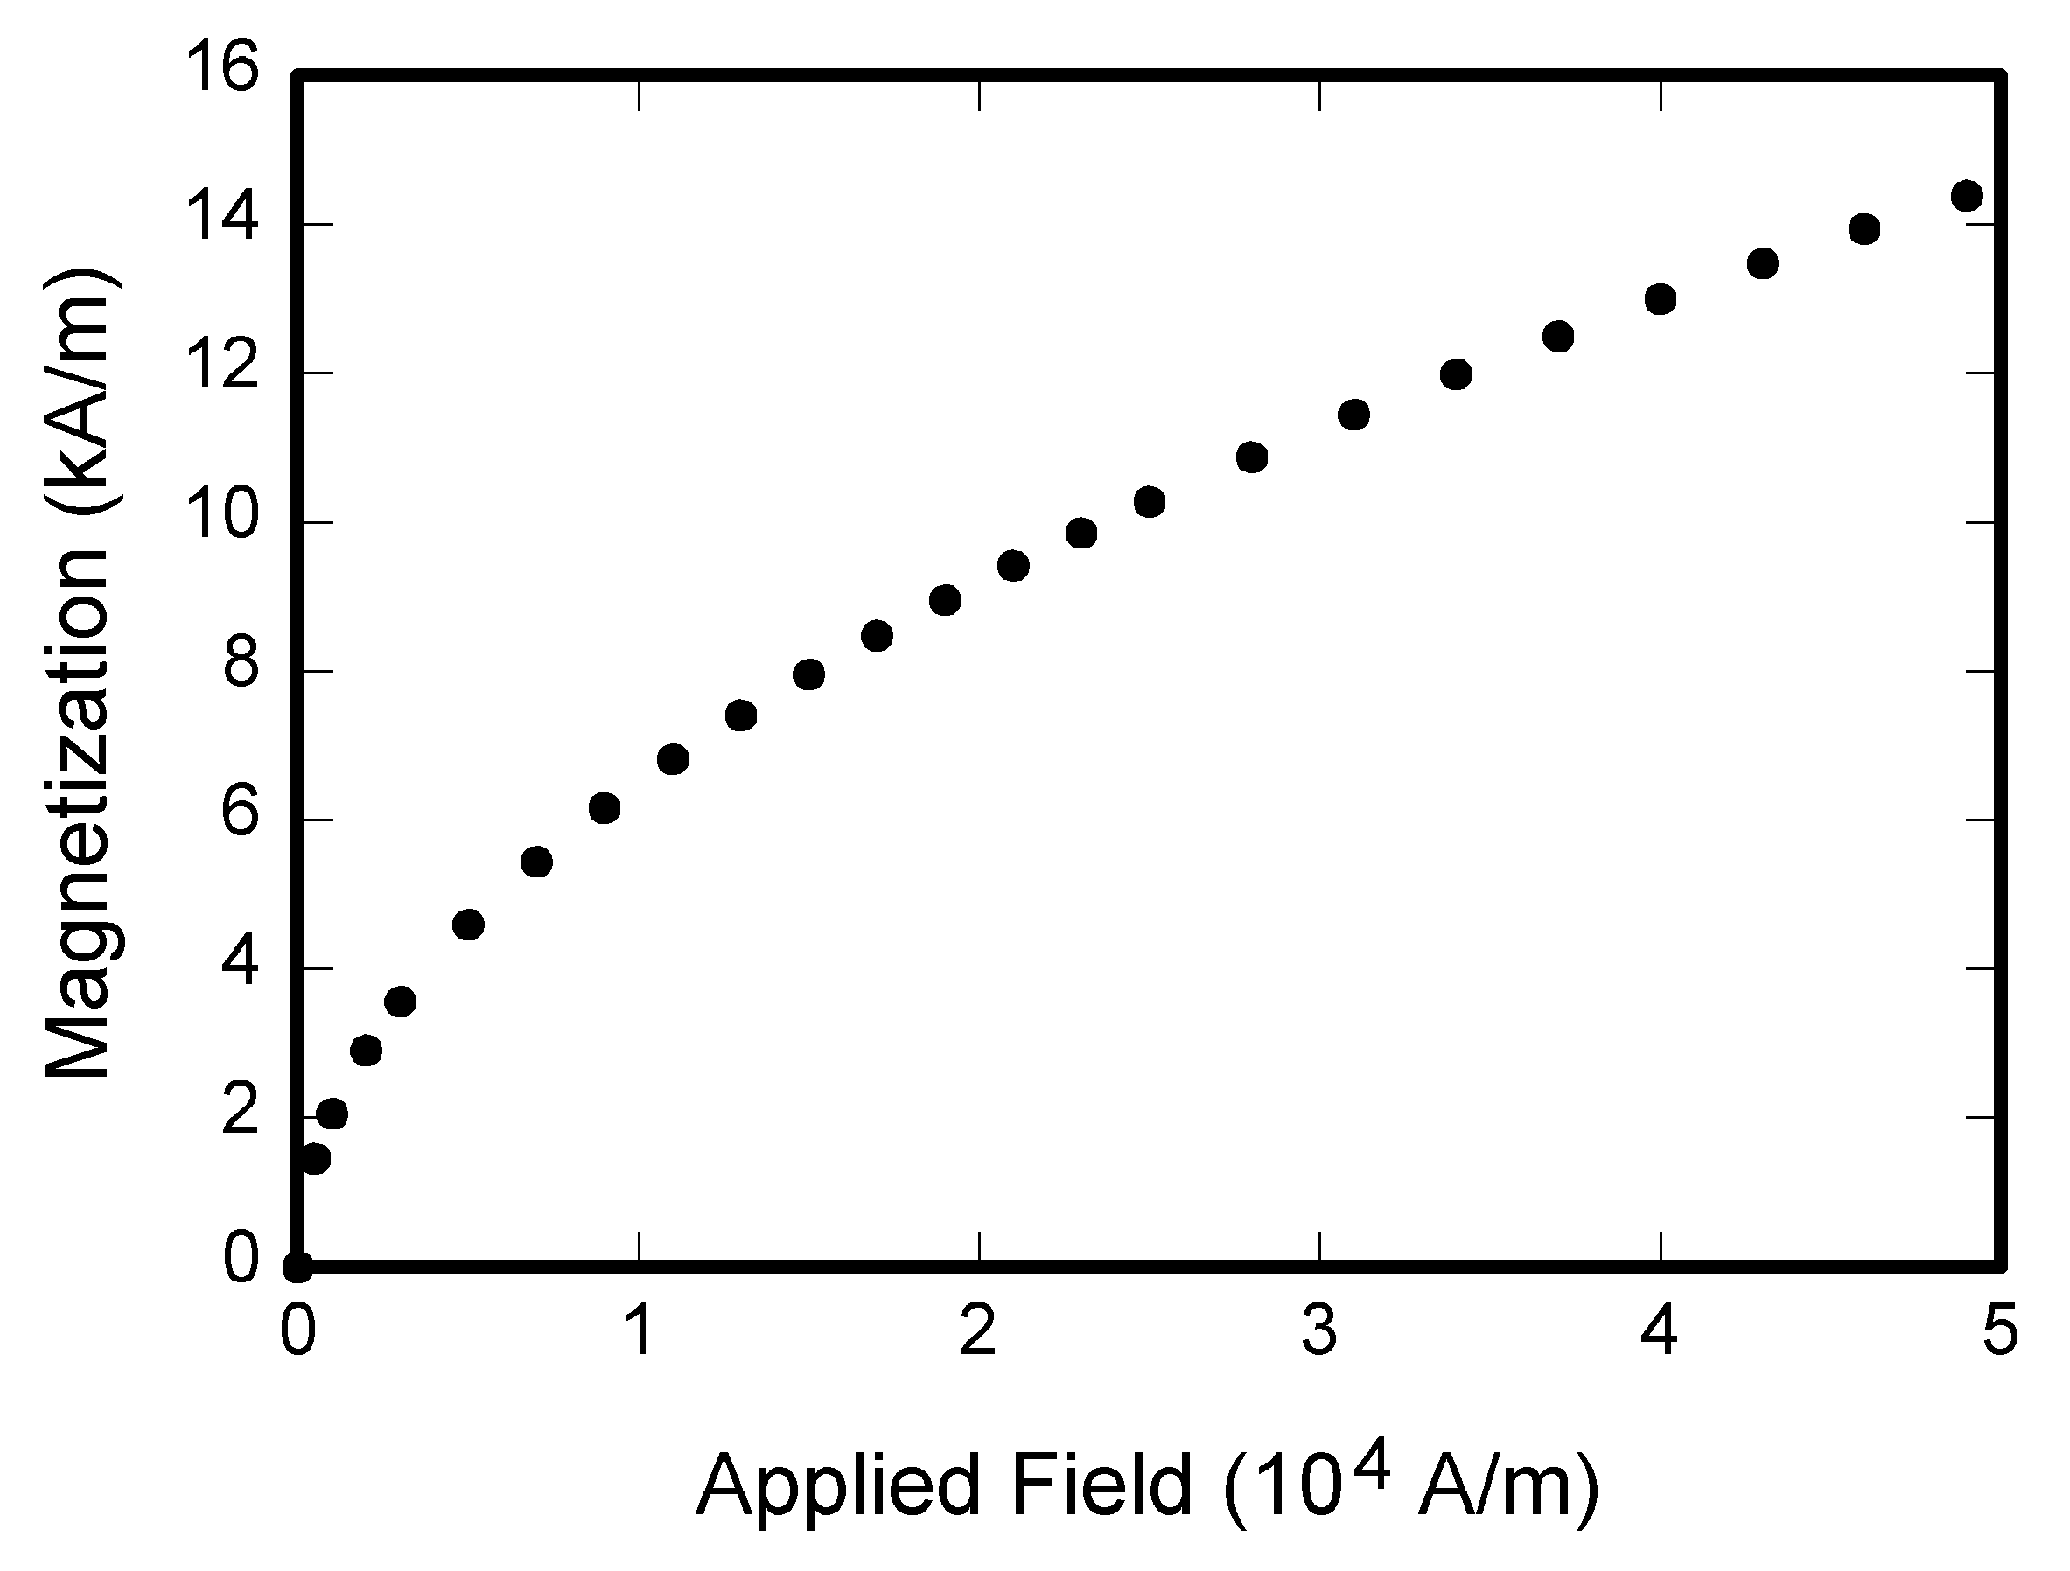
\includegraphics[width=0.45\textwidth]{images/fig1.png}} 
\caption{System comparison: Natural leaf vs. artificial photoelectrochemical cell.}
\label{fig:artificial}
\end{figure}

\subsection{Bionic Approaches for Hydrogen Production}
% Grüne Wasserstoffproduktion
Discuss current state-of-the-art technologies and bionic engineering approaches for synthesizing solar fuels.

\section{Conclusion and Future Outlook}
Summarize the main biophysical mechanisms discussed. Conclude with an outlook on what challenges remain for engineers to fully replicate or even surpass natural photosynthesis in terms of efficiency and scalability.
\section*{Acknowledgment}
Optional: I would like to thank...

% RICHTIG: Nur die BibTeX-Befehle nutzen
\bibliographystyle{IEEEtran}
\bibliography{quellen}

\end{document}
